\documentclass[10pt,a4paper]{article}

\usepackage[margin=1.65cm]{geometry}
\usepackage[T1]{fontenc}
\usepackage[utf8]{inputenc}
\usepackage{lmodern}
\usepackage{microtype}
\usepackage{xcolor}
\usepackage{amsmath}
\usepackage{booktabs}
\usepackage{tabularx}
\usepackage{array}
\usepackage{enumitem}
\usepackage{tikz}
\usetikzlibrary{arrows.meta,positioning,calc,fit,shapes.geometric}
\usepackage{hyperref}
\usepackage{xurl}
\hypersetup{colorlinks=true, linkcolor=blue!55!black, urlcolor=blue!55!black, citecolor=blue!55!black}
\setlength{\parindent}{0pt}
\setlength{\parskip}{5pt}
\renewcommand{\arraystretch}{1.16}

\definecolor{devblue}{HTML}{DDEEFF}
\definecolor{mainorange}{HTML}{FFE7C2}
\definecolor{stylepurple}{HTML}{EEE2FF}
\definecolor{contentgreen}{HTML}{E1F5E4}
\definecolor{sharedgray}{HTML}{F2F4F7}
\definecolor{alertred}{HTML}{FDE2E2}
\definecolor{ink}{HTML}{203040}

\newcommand{\dev}{\textcolor{blue!65!black}{\textbf{DEV}}}
\newcommand{\mainbranch}{\textcolor{orange!55!black}{\textbf{MAIN}}}
\newcommand{\code}[2]{\href{#1}{\texttt{#2}}}
\newcommand{\paper}[2]{\href{#1}{#2}}
\newcommand{\srcmainG}{\code{https://github.com/rquq/HGGAN_test/blob/main/networks/BigGAN_networks.py}{MAIN BigGAN\_networks.py}}
\newcommand{\srcdevG}{\code{https://github.com/rquq/HGGAN_test/blob/dev/networks/BigGAN_networks.py}{DEV BigGAN\_networks.py}}
\newcommand{\srctexture}{\code{https://github.com/rquq/HGGAN_test/blob/main/networks/texture_generator.py}{MAIN texture\_generator.py}}
\newcommand{\srcfusion}{\code{https://github.com/rquq/HGGAN_test/blob/dev/networks/fusion.py}{shared fusion.py}}
\newcommand{\srccfg}{\code{https://github.com/rquq/HGGAN_test/blob/dev/configs/gan_iam.yml}{shared gan\_iam.yml}}

\tikzset{
  flow/.style={-{Latex[length=2.0mm,width=1.3mm]}, thick, draw=ink},
  skipflow/.style={-{Latex[length=2.0mm,width=1.3mm]}, thick, draw=gray!65, dashed},
  tinyflow/.style={-{Latex[length=1.5mm,width=1.0mm]}, semithick, draw=ink},
  box/.style={draw=ink, rounded corners=2pt, minimum height=8mm, align=center, inner sep=3.2pt, font=\footnotesize},
  devbox/.style={box, fill=devblue},
  mainbox/.style={box, fill=mainorange},
  stylebox/.style={box, fill=stylepurple},
  contentbox/.style={box, fill=contentgreen},
  sharedbox/.style={box, fill=sharedgray},
  warnbox/.style={box, fill=alertred},
  smallbox/.style={box, minimum height=6.5mm, font=\scriptsize, inner sep=2.5pt},
  label/.style={font=\scriptsize, text=ink, align=center}
}

\title{\vspace{-1.5em}\textbf{Generator comparison: MAIN versus DEV}\\[-0.25em]
\large Exact implementation delta, paper provenance, and complete architecture diagrams}
\author{HGGAN\_test --- current branch source comparison}
\date{20 August 2026}

\begin{document}
\maketitle
\vspace{-1.0em}

\section*{Executive conclusion}

The current \mainbranch{} Generator is \emph{not} a replacement architecture for \dev.  It is the same Generator from text/style fusion through four conditioned GBlocks, plus one small, terminal residual head:
\[
  \text{MAIN output}=\tanh\big(\text{DEV base logits}+\text{bounded style--frequency detail}\big).
\]
Everything upstream of this addition is shared: text embedding, the full three-stage style--content/allograph fusion module, the $8$ style tokens ($1$ global + $7$ local), the $32$-D token size, the per-GBlock global-style projections, the $64$-wide GBlock decoder, and the $64\times32L$ output geometry.  In particular, the fusion code and Generator YAML are identical across the branches.  The intended role of MAIN's addition is texture and pen-edge refinement, not word geometry, character layout, or a new loss.

This is therefore an \emph{experimental quality-capacity trade}: MAIN adds only about $37{,}058$ Generator parameters (approximately $4.022$M vs. $3.985$M) but introduces a second high-resolution activation path.  It is plausible for this to improve fine strokes, yet it is not automatically ``better.''  If validation FID is worse or the samples acquire stray short lines, DEV remains the safer model; the bounded residual limits damage but cannot guarantee a gain.

\section{Scope, nomenclature, and method}

This report compares the active Generator source in the current \dev{} and \mainbranch{} branches.  ``Difference'' below means a source-level Generator difference, not a difference in discriminator, data pipeline, checkpoint, optimizer state, or training schedule.

\begin{itemize}[leftmargin=1.45em,itemsep=2pt]
  \item \textbf{DEV base Generator:} a conditional BigGAN-style convolutional decoder for handwriting.
  \item \textbf{MAIN Generator:} DEV base Generator $+$ \texttt{StyleFrequencyRefinement} immediately before the final \texttt{tanh}.
  \item \textbf{Style tokens:} $z\in\mathbb{R}^{B\times8\times32}$, where $z_0$ is the explicit global style token and $z_{1:7}$ are local tokens.
  \item \textbf{Text:} character ids $y\in\{0,\ldots,79\}^{B\times L}$, with valid lengths $y_{\mathrm{lens}}$.  $L$ is the padded character-sequence length.
  \item \textbf{Paper provenance:} a cited paper documents the underlying idea, \emph{not} necessarily a line-for-line reproduction.  The exact composition, bounds, style descriptor, and initialization are project-specific adaptations.  This distinction matters when interpreting expected behavior.
\end{itemize}

\subsection*{Exact source comparison}

The direct diff is compact:

\begin{center}
\small
\begin{tabularx}{\textwidth}{@{}p{0.19\textwidth}X p{0.23\textwidth}@{}}
\toprule
Location & \dev{} & \mainbranch{} \\
\midrule
Imports & No texture module. & Imports \texttt{StyleFrequencyRefinement}. \\
Construction & Builds only \texttt{output\_layer = BN $\rightarrow$ ReLU $\rightarrow$ SNConv}. & Builds the same \texttt{output\_layer}, then adds \texttt{texture\_refinement(channels=64, style\_dim=32, output\_channels=1)}. \\
Output path & \texttt{tanh(output\_layer(h))}. & \texttt{tanh(output\_layer(h) + texture\_refinement(h, z))}. \\
Shared items & \multicolumn{2}{l}{Same \srcfusion{}; same \srccfg{}; same GBlock schedule; no configured G self-attention (\texttt{G\_attn: '0'}).} \\
\bottomrule
\end{tabularx}
\end{center}

The relevant code is \srcdevG{} lines 192--257, \srcmainG{} lines 193--268, and \srctexture{} lines 1--156.  The configuration that fixes the shared dimensions is \srccfg{} lines 150--182 and 236--241.

\section{The shared Generator: what both branches already do}

Both Generators are rooted in the conditional-residual design direction of \paper{https://arxiv.org/abs/1809.11096}{BigGAN}---spectral-normalized layers, conditional normalization inside residual upsampling blocks, and a high-capacity conditional generator.  The implementation is handwriting-specific: text characters create a sequence of vertical seed strips, while style is injected both into character-level fusion and into every GBlock.

\begin{center}
\resizebox{0.98\textwidth}{!}{%
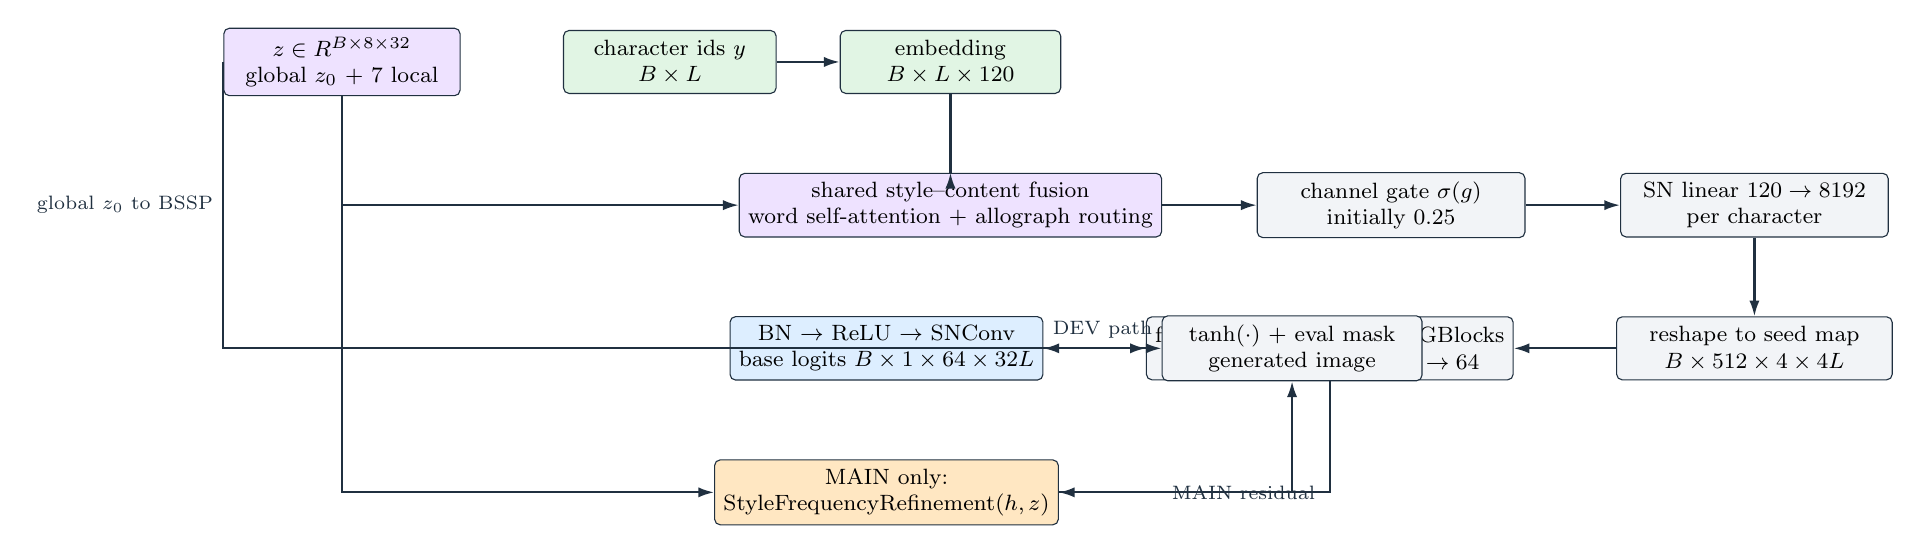
\begin{tikzpicture}[node distance=8mm and 8mm]
  \node[stylebox, minimum width=30mm] (z) {$z\in\mathbb{R}^{B\times8\times32}$\\global $z_0$ + 7 local};
  \node[contentbox, minimum width=27mm, right=13mm of z] (y) {character ids $y$\\$B\times L$};
  \node[contentbox, minimum width=28mm, right=of y] (emb) {embedding\\$B\times L\times120$};
  \node[stylebox, minimum width=38mm, below=10mm of emb] (fusion) {shared style--content fusion\\word self-attention + allograph routing};
  \node[sharedbox, minimum width=34mm, right=12mm of fusion] (gate) {channel gate $\sigma(g)$\\initially $0.25$};
  \node[sharedbox, minimum width=34mm, right=12mm of gate] (linear) {SN linear $120\rightarrow8192$\\per character};
  \node[sharedbox, minimum width=35mm, below=10mm of linear] (seed) {reshape to seed map\\$B\times512\times4\times4L$};
  \node[sharedbox, minimum width=43mm, left=13mm of seed] (blocks) {four conditioned residual GBlocks\\$512\rightarrow256\rightarrow128\rightarrow64\rightarrow64$};
  \node[devbox, minimum width=33mm, left=13mm of blocks] (base) {BN $\rightarrow$ ReLU $\rightarrow$ SNConv\\base logits $B\times1\times64\times32L$};
  \node[mainbox, minimum width=42mm, below=10mm of base] (detail) {MAIN only:\\StyleFrequencyRefinement$(h,z)$};
  \node[sharedbox, minimum width=33mm, right=15mm of base] (tanh) {$\tanh(\cdot)$ + eval mask\\generated image};

  \draw[flow] (y) -- (emb);
  \draw[flow] (emb.south) |- (fusion.north);
  \draw[flow] (z.south) |- (fusion.west);
  \draw[flow] (fusion) -- (gate);
  \draw[flow] (gate) -- (linear);
  \draw[flow] (linear.south) -- (seed.north);
  \draw[flow] (seed.west) -- (blocks.east);
  \draw[flow] (blocks) -- (base);
  \draw[flow] (base) -- node[label,above]{DEV path} (tanh);
  \draw[flow] (z.west) |- node[label,pos=.25,left]{global $z_0$ to BSSP} (blocks.west);
  \draw[flow] (blocks.south) |- (detail.east);
  \draw[flow] (z.south) |- (detail.west);
  \draw[flow] (detail.east) -| node[label,pos=.22,right]{MAIN residual} (tanh.south);
\end{tikzpicture}}
\end{center}

\subsection*{Shared tensor flow, in detail}

\begin{enumerate}[leftmargin=1.55em,itemsep=3pt]
  \item \textbf{Global style to every GBlock.}  Only $z_0$ enters the Block-Specific Style Projection (BSSP).  Four distinct $32\rightarrow32\rightarrow32$ projections provide the conditional-BN signal for the four decoder blocks.  Local style cannot bypass the aligned fusion path.
  \item \textbf{Content--style mixing.}  Text embeddings have shape $B\times L\times120$.  The shared fusion module produces fused content of the same shape; a learned channelwise gate starts at $0.25$, so the initial mixture retains a strong original-content route:
  \[
    y_{\mathrm{mixed}}=y_{\mathrm{content}}+\sigma(g)\big(y_{\mathrm{fused}}-y_{\mathrm{content}}\big).
  \]
  \item \textbf{Strip seed.}  The mixed representation is linearly expanded from $120$ to $512\times4\times4=8192$ values per character, then re-arranged to $B\times512\times4\times4L$.  Each character begins as a four-pixel-wide strip.
  \item \textbf{Decoder.}  The four GBlocks have channel schedule $512\rightarrow256\rightarrow128\rightarrow64\rightarrow64$ and upsample factors $(2,1),(2,2),(2,2),(2,2)$.  This yields height $4\rightarrow8\rightarrow16\rightarrow32\rightarrow64$ and width $4L\rightarrow4L\rightarrow8L\rightarrow16L\rightarrow32L$.  The current \texttt{G\_attn: '0'} means neither branch enables a Generator self-attention block.
  \item \textbf{Shared image head.}  A final batch-normalization, ReLU, and spectral-normalized $3\times3$ convolution map $64$ feature channels to one grayscale logit channel.  DEV passes it directly to \texttt{tanh}; MAIN adds the residual described next.
\end{enumerate}

\section{MAIN-only change 1 --- terminal residual topology}

\textbf{What changes.}  MAIN keeps the complete DEV decoder and adds an image-logit residual at the very end.  It does \emph{not} alter the content route, GBlock count, channel widths, upsampling schedule, fusion, or output resolution.

\textbf{Code.}  Construction: \href{https://github.com/rquq/HGGAN_test/blob/main/networks/BigGAN_networks.py\#L195-L213}{MAIN lines 195--213}; forward addition: \href{https://github.com/rquq/HGGAN_test/blob/main/networks/BigGAN_networks.py\#L255-L259}{MAIN lines 255--259}; DEV terminal path: \href{https://github.com/rquq/HGGAN_test/blob/dev/networks/BigGAN_networks.py\#L247-L248}{DEV lines 247--248}.

\textbf{Paper connection.}  The shared conditional residual decoder is in the design lineage of \paper{https://arxiv.org/abs/1809.11096}{Brock et al., BigGAN (2019)}.  Adding a residual frequency-focused output head is a project-specific adaptation; it is not claimed to be a literal BigGAN layer.

\begin{center}
\resizebox{0.88\textwidth}{!}{%
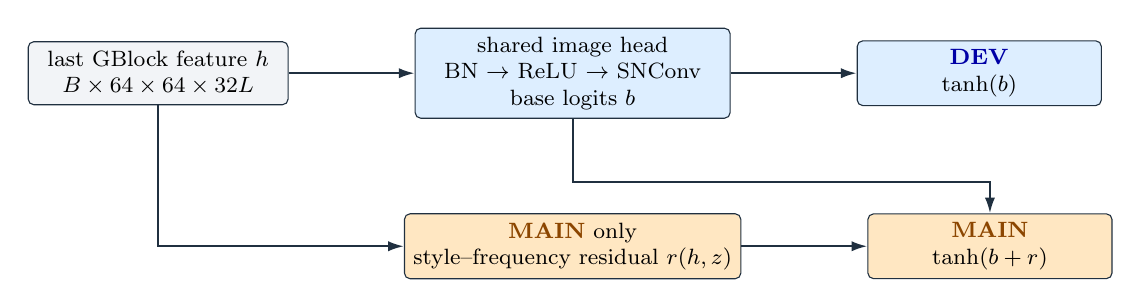
\begin{tikzpicture}[node distance=11mm and 16mm]
  \node[sharedbox, minimum width=33mm] (h) {last GBlock feature $h$\\$B\times64\times64\times32L$};
  \node[devbox, minimum width=40mm, right=of h] (head) {shared image head\\BN $\rightarrow$ ReLU $\rightarrow$ SNConv\\base logits $b$};
  \node[devbox, minimum width=31mm, right=of head] (devout) {\dev{}\\$\tanh(b)$};
  \node[mainbox, minimum width=41mm, below=12mm of head] (refine) {\mainbranch{} only\\style--frequency residual $r(h,z)$};
  \node[mainbox, minimum width=31mm, right=of refine] (mainout) {\mainbranch{}\\$\tanh(b+r)$};
  \draw[flow] (h) -- (head);
  \draw[flow] (head) -- (devout);
  \draw[flow] (h.south) |- (refine.west);
  \draw[flow] (head.south) -- ++(0,-0.8) -| (mainout.north);
  \draw[flow] (refine) -- (mainout);
\end{tikzpicture}}
\end{center}

\textbf{Why this is structurally conservative.}  $r$ is added to logits, then one \texttt{tanh} is applied.  MAIN does not stack a second image nonlinearity, nor does it overwrite the base image.  This preserves a direct path from the proven DEV head to the image.  The risk remains that an additive residual can create coherent but unwanted pen-like marks if its frequency content is poorly calibrated.

\section{MAIN-only change 2 --- style-distribution descriptor and bounded affine modulation}

\textbf{What changes.}  MAIN's refinement head reads all style tokens, rather than only the global token.  It builds one $96$-D descriptor from (i) the global token, (ii) the mean of seven local tokens, and (iii) their per-dimension standard deviation:
\[
 d=\big[z_0\ ;\ \mu(z_{1:7})\ ;\ \sigma(z_{1:7})\big]\in\mathbb{R}^{96}.
\]
It projects $d$ to a per-channel scale and shift for the $64$-channel detail feature.  Both raw affine terms are bounded with \texttt{tanh} at magnitude $0.15$.  The scale is then RMS-normalized across channels, keeping a writer's style strength from simply changing the total feature energy.

\textbf{Code.}  Descriptor: \href{https://github.com/rquq/HGGAN_test/blob/main/networks/texture_generator.py\#L100-L114}{texture\_generator.py lines 100--114}; modulation and scale normalization: \href{https://github.com/rquq/HGGAN_test/blob/main/networks/texture_generator.py\#L116-L145}{lines 116--145}.

\textbf{Paper connection.}  This is closest in spirit to the modulation/demodulation stability goal of \paper{https://arxiv.org/abs/1912.04958}{Karras et al., StyleGAN2 (2020)}, but it is \emph{feature} RMS normalization rather than StyleGAN2's weight demodulation.  The global--mean--standard-deviation descriptor itself is a project-specific summary of the existing local slots.

\begin{center}
\resizebox{0.95\textwidth}{!}{%
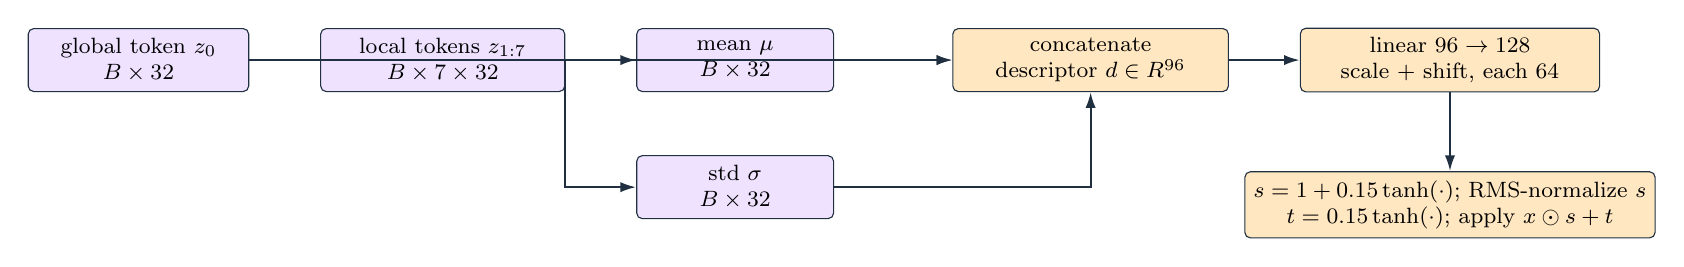
\begin{tikzpicture}[node distance=8mm and 9mm]
  \node[stylebox, minimum width=28mm] (global) {global token $z_0$\\$B\times32$};
  \node[stylebox, minimum width=31mm, right=of global] (local) {local tokens $z_{1:7}$\\$B\times7\times32$};
  \node[stylebox, minimum width=25mm, right=of local] (mean) {mean $\mu$\\$B\times32$};
  \node[stylebox, minimum width=25mm, below=of mean] (std) {std $\sigma$\\$B\times32$};
  \node[mainbox, minimum width=35mm, right=15mm of mean] (desc) {concatenate\\descriptor $d\in\mathbb{R}^{96}$};
  \node[mainbox, minimum width=38mm, right=of desc] (affine) {linear $96\rightarrow128$\\scale + shift, each $64$};
  \node[mainbox, minimum width=47mm, below=10mm of affine] (mod) {$s=1+0.15\tanh(\cdot)$; RMS-normalize $s$\\$t=0.15\tanh(\cdot)$; apply $x\odot s+t$};
  \draw[flow] (local) -- (mean);
  \draw[flow] (local.east) |- (std.west);
  \draw[flow] (global.east) -- ++(0.5,0) |- (desc.west);
  \draw[flow] (mean.east) -- (desc.west);
  \draw[flow] (std.east) -| (desc.south);
  \draw[flow] (desc) -- (affine);
  \draw[flow] (affine.south) -- (mod.north);
\end{tikzpicture}}
\end{center}

\textbf{Interpretation.}  The mean gives a consensus local style; the standard deviation encodes how heterogeneous the local slots are.  Thus the detail head can distinguish, for example, a uniformly smooth writer from one whose local slots represent several stroke variants.  This extra conditioning exists only in the texture residual; the shared allograph routing still controls the main character-level geometry.

\section{MAIN-only change 3 --- gated oriented depthwise texture branches}

\textbf{What changes.}  From the final $64$-channel feature map, MAIN computes three depthwise convolutional candidates: horizontal $(1\times7)$, vertical $(7\times1)$, and compact local $(3\times3)$.  A style-conditioned $96\rightarrow(3\times64)$ linear layer produces a softmax over the three candidates for every channel.  The selected mixture is then passed through SiLU and a $1\times1$ channel mixer.

\textbf{Code.}  Branch construction: \href{https://github.com/rquq/HGGAN_test/blob/main/networks/texture_generator.py\#L59-L84}{lines 59--84}; softmax gate and mixture: \href{https://github.com/rquq/HGGAN_test/blob/main/networks/texture_generator.py\#L126-L140}{lines 126--140}.

\textbf{Paper connection.}  The separated square and orthogonal band depthwise branches are inspired by \paper{https://arxiv.org/abs/2303.16900}{Yu et al., InceptionNeXt (2023)}, which decomposes a large depthwise spatial operation into parallel compact and directional branches.  The adaptive gated aggregation motivation is from \paper{https://arxiv.org/abs/2211.03295}{Li et al., MogaNet (2022)}.  MAIN uses a lighter three-branch, per-channel mixture tailored to $64\times32L$ handwriting features; it does not reproduce either paper's block exactly.

\begin{center}
\resizebox{0.96\textwidth}{!}{%
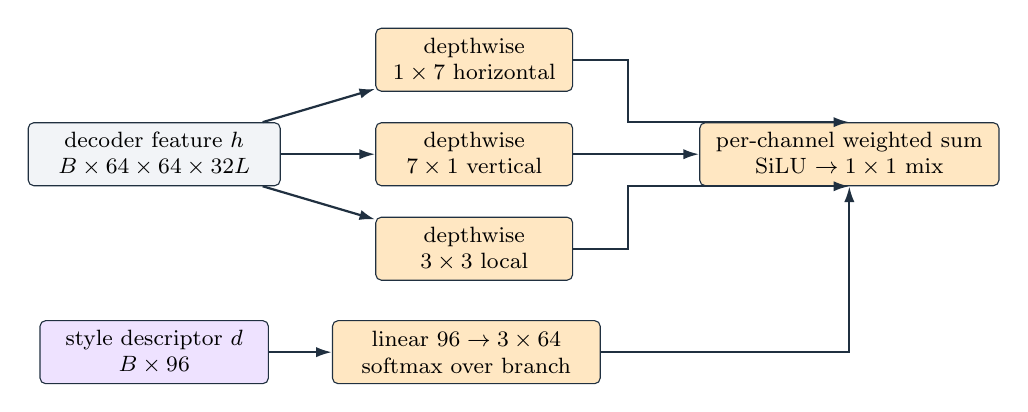
\begin{tikzpicture}[node distance=8mm and 8mm]
  \node[sharedbox, minimum width=32mm] (feat) {decoder feature $h$\\$B\times64\times64\times32L$};
  \node[mainbox, minimum width=25mm, right=12mm of feat, yshift=12mm] (hor) {depthwise\\$1\times7$ horizontal};
  \node[mainbox, minimum width=25mm, right=12mm of feat] (ver) {depthwise\\$7\times1$ vertical};
  \node[mainbox, minimum width=25mm, right=12mm of feat, yshift=-12mm] (loc) {depthwise\\$3\times3$ local};
  \node[stylebox, minimum width=29mm, below=17mm of feat] (desc2) {style descriptor $d$\\$B\times96$};
  \node[mainbox, minimum width=34mm, right=of desc2] (gate2) {linear $96\rightarrow3\times64$\\softmax over branch};
  \node[mainbox, minimum width=38mm, right=16mm of ver] (mix) {per-channel weighted sum\\SiLU $\rightarrow1\times1$ mix};
  \draw[flow] (feat) -- (hor);
  \draw[flow] (feat) -- (ver);
  \draw[flow] (feat) -- (loc);
  \draw[flow] (desc2) -- (gate2);
  \draw[flow] (gate2.east) -| (mix.south);
  \draw[flow] (hor.east) -- ++(7mm,0) |- (mix.north);
  \draw[flow] (ver) -- (mix);
  \draw[flow] (loc.east) -- ++(7mm,0) |- (mix.south);
\end{tikzpicture}}
\end{center}

\textbf{Interpretation.}  The three candidates are directional texture hypotheses, not explicit handwriting primitives.  The horizontal branch can emphasize baseline/pen-edge continuity; vertical can support ascender/descender edges; local can preserve compact curvature.  A softmax mixture avoids blindly summing all three.  Nevertheless, these branches operate at the final, high-resolution feature stage, so poorly regularized selection can still look like extra micro-strokes rather than genuine allographs.

\section{MAIN-only change 4 --- Global Response Normalization (GRN)}

\textbf{What changes.}  After the channel mix, MAIN applies GRN:
\[
 r_c=\lVert x_c\rVert_2\quad\text{over spatial dimensions},\qquad
 \hat r_c=\frac{r_c}{\operatorname{mean}_c(r_c)+\epsilon},\qquad
 \operatorname{GRN}(x)=x+\gamma(x\odot\hat r)+\beta.
\]
Here $\gamma$ and $\beta$ are learned $1\times64\times1\times1$ parameters and are initialized to zero, so GRN begins as an identity transformation.

\textbf{Code.}  GRN implementation: \href{https://github.com/rquq/HGGAN_test/blob/main/networks/texture_generator.py\#L17-L34}{texture\_generator.py lines 17--34}; identity initialization: \href{https://github.com/rquq/HGGAN_test/blob/main/networks/texture_generator.py\#L90-L98}{lines 90--98}.

\textbf{Paper connection.}  This is the Global Response Normalization idea from \paper{https://arxiv.org/abs/2301.00808}{Woo et al., ConvNeXt V2 (2023)}.  In that work, GRN encourages inter-channel feature competition.  MAIN places it only in the texture residual instead of across the full Generator.

\begin{center}
\resizebox{0.88\textwidth}{!}{%
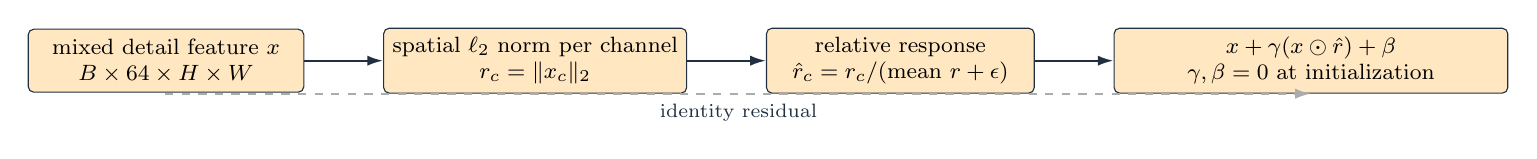
\begin{tikzpicture}[node distance=9mm and 10mm]
  \node[mainbox, minimum width=35mm] (x) {mixed detail feature $x$\\$B\times64\times H\times W$};
  \node[mainbox, minimum width=33mm, right=of x] (norm) {spatial $\ell_2$ norm per channel\\$r_c=\Vert x_c\Vert_2$};
  \node[mainbox, minimum width=34mm, right=of norm] (rel) {relative response\\$\hat r_c=r_c/(\mathrm{mean}\ r+\epsilon)$};
  \node[mainbox, minimum width=50mm, right=of rel] (out) {$x+\gamma(x\odot\hat r)+\beta$\\$\gamma,\beta=0$ at initialization};
  \draw[flow] (x) -- (norm);
  \draw[flow] (norm) -- (rel);
  \draw[flow] (rel) -- (out);
  \draw[skipflow] (x.south) |- node[label,pos=.75,below]{identity residual} (out.south);
\end{tikzpicture}}
\end{center}

\textbf{Interpretation.}  GRN is not a style encoder and not a spatial attention layer.  It rescales channels relative to the feature-map-wide response, then learns how strongly to use that information.  Because this is a high-resolution feature map, the spatial norm reduction itself is cheap relative to a full attention map, while the surrounding branch activations are the more meaningful memory cost.

\section{MAIN-only change 5 --- high-pass residual and capped detail gain}

\textbf{What changes.}  MAIN converts the modulated feature to a one-channel raw detail image, subtracts a reflect-padded $3\times3$ local average, then applies a learned but bounded gain:
\[
 d_{\mathrm{HP}}=d_{\mathrm{raw}}-\operatorname{AvgPool}_{3\times3}\!\left(\operatorname{ReflectPad}(d_{\mathrm{raw}})\right),\qquad
 r=0.15\,\sigma(a)\,d_{\mathrm{HP}}.
\]
The gain begins at $0.03$ and remains strictly below $0.15$.  This makes the new head explicitly a local-detail residual rather than another generator for low-frequency word shape.

\textbf{Code.}  Detail projection and high-pass residual: \href{https://github.com/rquq/HGGAN_test/blob/main/networks/texture_generator.py\#L145-L153}{texture\_generator.py lines 145--153}; gain bounds: \href{https://github.com/rquq/HGGAN_test/blob/main/networks/texture_generator.py\#L45-L57}{lines 45--57}.

\textbf{Paper connection.}  Frequency-aware GAN work motivates separating high-frequency detail from coarse image structure, e.g. \paper{https://arxiv.org/abs/2207.07288}{WaveGAN (2022)} and \paper{https://arxiv.org/abs/2210.05461}{FreGAN (2022)}.  MAIN's reflect-pad local-average subtraction and $0.15\sigma(a)$ cap are project-specific safeguards, not an implementation copied from those papers.

\begin{center}
\resizebox{0.93\textwidth}{!}{%
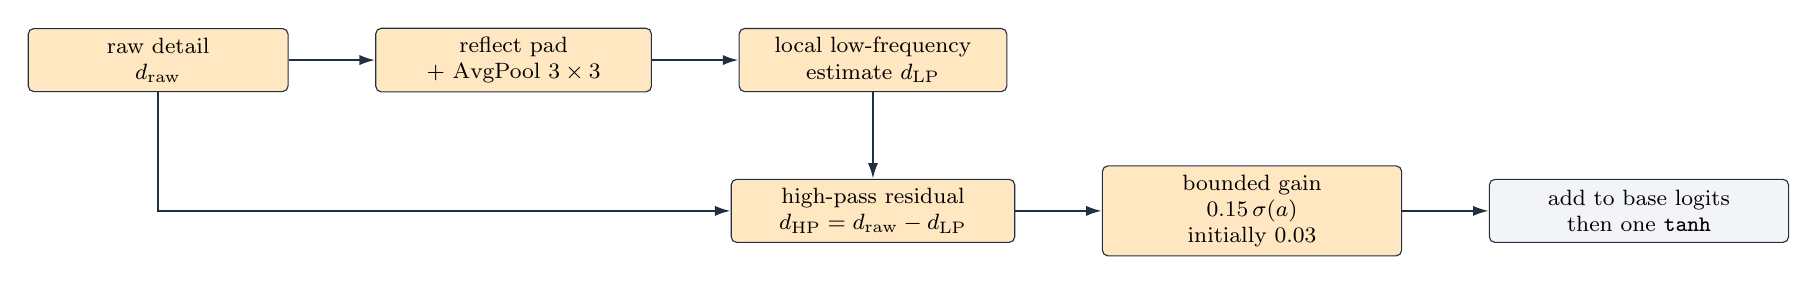
\begin{tikzpicture}[node distance=9mm and 11mm]
  \node[mainbox, minimum width=33mm] (raw) {raw detail\\$d_{\mathrm{raw}}$};
  \node[mainbox, minimum width=35mm, right=of raw] (pad) {reflect pad\\$+$ AvgPool $3\times3$};
  \node[mainbox, minimum width=34mm, right=of pad] (low) {local low-frequency\\estimate $d_{\mathrm{LP}}$};
  \node[mainbox, minimum width=36mm, below=11mm of low] (hp) {high-pass residual\\$d_{\mathrm{HP}}=d_{\mathrm{raw}}-d_{\mathrm{LP}}$};
  \node[mainbox, minimum width=38mm, right=of hp] (gain) {bounded gain\\$0.15\,\sigma(a)$\\initially $0.03$};
  \node[sharedbox, minimum width=38mm, right=of gain] (sum) {add to base logits\\then one \texttt{tanh}};
  \draw[flow] (raw) -- (pad);
  \draw[flow] (pad) -- (low);
  \draw[flow] (low.south) -- (hp.north);
  \draw[flow] (raw.south) |- (hp.west);
  \draw[flow] (hp) -- (gain);
  \draw[flow] (gain) -- (sum);
\end{tikzpicture}}
\end{center}

\textbf{Interpretation and failure mode.}  This block deliberately cannot directly alter the broad character skeleton through its low-frequency band.  However, high-pass does not mean ``always correct'': a high-pass residual can still synthesize short, sharp, spurious lines.  The cap is therefore a stability aid, not a guarantee against artifacts.  Tracking the learned \texttt{detail\_gain} and sampling at fixed text/style pairs is the cleanest way to judge whether this head helps.

\section{Complete Generator diagram}

The following diagram is the complete active Generator.  Solid gray/blue/green/purple blocks are shared by DEV and MAIN.  Orange blocks are MAIN-only.  There are no hidden G self-attention blocks in the current configuration.

\begin{center}
\resizebox{0.98\textwidth}{!}{%
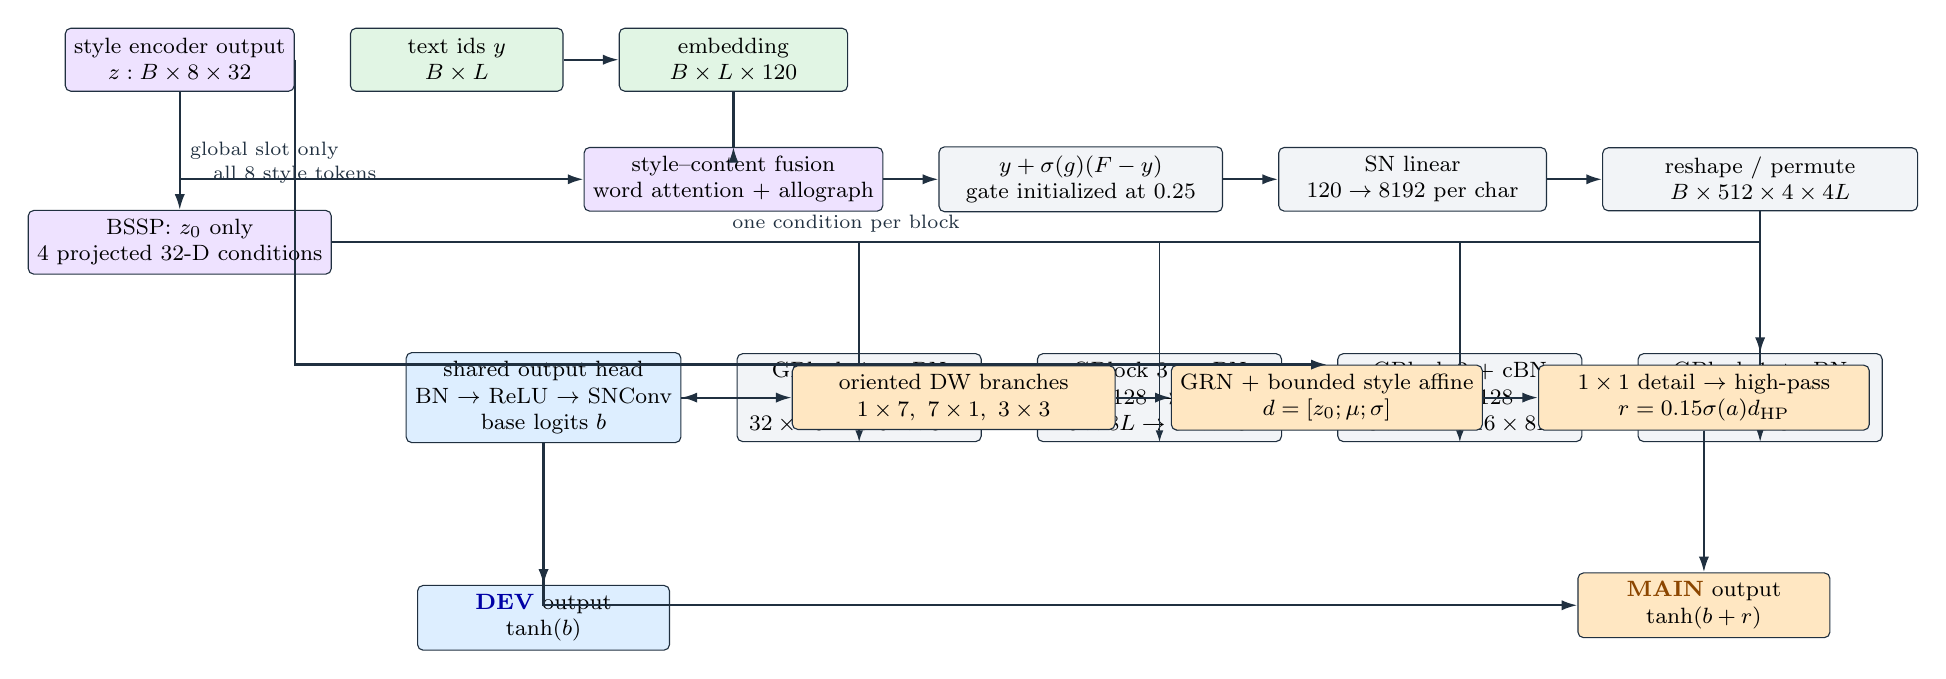
\begin{tikzpicture}[node distance=7mm and 7mm]
  % Inputs and fusion
  \node[stylebox, minimum width=27mm] (Z) {style encoder output\\$z:B\times8\times32$};
  \node[contentbox, minimum width=27mm, right=of Z] (Y) {text ids $y$\\$B\times L$};
  \node[contentbox, minimum width=29mm, right=of Y] (E) {embedding\\$B\times L\times120$};
  \node[stylebox, minimum width=34mm, below=of E] (F) {style--content fusion\\word attention + allograph};
  \node[sharedbox, minimum width=36mm, right=of F] (M) {$y+\sigma(g)(F-y)$\\gate initialized at $0.25$};
  \node[sharedbox, minimum width=34mm, right=of M] (L) {SN linear\\$120\rightarrow8192$ per char};
  \node[sharedbox, minimum width=40mm, right=of L] (S) {reshape / permute\\$B\times512\times4\times4L$};
  \draw[flow] (Y) -- (E);
  \draw[flow] (E.south) |- (F.north);
  \draw[flow] (Z.south) |- (F.west);
  \draw[flow] (F) -- (M);
  \draw[flow] (M) -- (L);
  \draw[flow] (L) -- (S);

  % BSSP route
  \node[stylebox, minimum width=34mm, below=15mm of Z] (BSSP) {BSSP: $z_0$ only\\4 projected $32$-D conditions};
  \draw[flow] (Z.south) -- node[label,right]{global slot only} (BSSP.north);

  % Decoder
  \node[sharedbox, minimum width=31mm, below=18mm of S] (G1) {GBlock 1 + cBN\\$512\rightarrow256$\\$4\times4L\rightarrow8\times4L$};
  \node[sharedbox, minimum width=31mm, left=of G1] (G2) {GBlock 2 + cBN\\$256\rightarrow128$\\$8\times4L\rightarrow16\times8L$};
  \node[sharedbox, minimum width=31mm, left=of G2] (G3) {GBlock 3 + cBN\\$128\rightarrow64$\\$16\times8L\rightarrow32\times16L$};
  \node[sharedbox, minimum width=31mm, left=of G3] (G4) {GBlock 4 + cBN\\$64\rightarrow64$\\$32\times16L\rightarrow64\times32L$};
  \node[devbox, minimum width=33mm, left=of G4] (H) {shared output head\\BN $\rightarrow$ ReLU $\rightarrow$ SNConv\\base logits $b$};
  \draw[flow] (S.south) -- (G1.north);
  \draw[flow] (G1) -- (G2);
  \draw[flow] (G2) -- (G3);
  \draw[flow] (G3) -- (G4);
  \draw[flow] (G4) -- (H);
  \draw[flow] (BSSP.east) -| node[label,pos=.18,above]{one condition per block} (G1.south);
  \draw[tinyflow] (BSSP.east) -| (G2.south);
  \draw[tinyflow] (BSSP.east) -| (G3.south);
  \draw[tinyflow] (BSSP.east) -| (G4.south);

  % Outputs
  \node[devbox, minimum width=32mm, below=18mm of H] (Dout) {\dev{} output\\$\tanh(b)$};
  \node[mainbox, minimum width=41mm, right=14mm of H] (R1) {oriented DW branches\\$1\times7,\ 7\times1,\ 3\times3$};
  \node[mainbox, minimum width=39mm, right=of R1] (R2) {GRN + bounded style affine\\$d=[z_0;\mu;\sigma]$};
  \node[mainbox, minimum width=42mm, right=of R2] (R3) {$1\times1$ detail $\rightarrow$ high-pass\\$r=0.15\sigma(a)d_{\mathrm{HP}}$};
  \node[mainbox, minimum width=32mm, below=18mm of R3] (Mout) {\mainbranch{} output\\$\tanh(b+r)$};
  \draw[flow] (H) -- (Dout);
  \draw[flow] (H) -- (R1);
  \draw[flow] (R1) -- (R2);
  \draw[flow] (R2) -- (R3);
  \draw[flow] (R3.south) -- (Mout.north);
  \draw[flow] (Z.east) |- node[label,pos=.22,above]{all $8$ style tokens} (R2.north);
  \draw[flow] (H.south) |- (Mout.west);
\end{tikzpicture}}
\end{center}

\section{What is shared versus what can explain a MAIN--DEV result gap}

\begin{center}
\small
\begin{tabularx}{\textwidth}{@{}p{0.28\textwidth}c c X@{}}
\toprule
Component & \dev{} & \mainbranch{} & Consequence for an experiment \\
\midrule
Style token count / dimension & $8\times32$ & $8\times32$ & Not a current G difference. \\
Style--content / allograph fusion & same & same & Not a current G difference; a FID gap is not caused by a branch-specific fusion implementation. \\
Text seed and GBlock decoder & same & same & Same geometry path and conditional-BN capacity. \\
Configured G attention & off & off & Neither model has an active Generator attention layer under \texttt{G\_attn: '0'}. \\
Image head & base logits only & base logits + texture residual & The sole active architecture delta. \\
Local-style statistical conditioning & no terminal use & mean/std descriptor in residual head & Adds writer-distribution information only to fine-detail synthesis. \\
Directional depthwise branches / GRN / high-pass & absent & present & Adds high-resolution activations and an additional artifact path, while keeping base image intact. \\
\bottomrule
\end{tabularx}
\end{center}

\subsection*{Practical reading of the two models}

\begin{itemize}[leftmargin=1.45em,itemsep=3pt]
  \item \textbf{DEV is the clean ablation baseline.}  Its output is entirely produced by the established text/style fusion plus conditioned GBlock decoder.  It has fewer moving parts and no terminal branch that can draw extra sharp marks.
  \item \textbf{MAIN is a targeted texture experiment.}  Its only added representational power is to choose and modulate directional high-frequency residual detail using the global/local style distribution.  It cannot by itself improve content alignment or character geometry except indirectly through joint training gradients.
  \item \textbf{A lower MAIN score would be informative, not paradoxical.}  MAIN has more capacity at precisely the stage where GANs can overfit high-frequency artifacts.  If the base is already strong, the correct ablation is to compare DEV, MAIN with the learned detail gain forced to zero, and MAIN normally---all at the same checkpoint selection policy and fixed validation seed.
  \item \textbf{Do not infer a paper-level guarantee.}  ConvNeXt V2, InceptionNeXt, MogaNet, StyleGAN2, WaveGAN, and FreGAN were developed and evaluated in different model/data regimes.  They motivate compact components; they do not establish that this exact handwritten-word residual will lower FID.
\end{itemize}

\section{References and direct links}

\begin{enumerate}[leftmargin=1.6em,itemsep=3pt]
  \item Brock, A., Donahue, J., \& Simonyan, K. \paper{https://arxiv.org/abs/1809.11096}{Large Scale GAN Training for High Fidelity Natural Image Synthesis (BigGAN), 2019}.  Shared conditional-GAN decoder lineage.
  \item Karras, T. et al. \paper{https://arxiv.org/abs/1912.04958}{Analyzing and Improving the Image Quality of StyleGAN (StyleGAN2), 2020}.  Modulation/demodulation stability context; MAIN's feature RMS normalization is an adaptation, not the paper's weight demodulation.
  \item Woo, S. et al. \paper{https://arxiv.org/abs/2301.00808}{ConvNeXt V2: Co-designing and Scaling ConvNets with Masked Autoencoders, 2023}.  Source of the GRN concept.
  \item Li, S. et al. \paper{https://arxiv.org/abs/2211.03295}{MogaNet: Multi-order Gated Aggregation Network, 2022}.  Gated multi-branch aggregation motivation.
  \item Yu, W. et al. \paper{https://arxiv.org/abs/2303.16900}{InceptionNeXt: When Inception Meets ConvNeXt, 2023}.  Parallel compact and orthogonal depthwise branch motivation.
  \item Yang, M. et al. \paper{https://arxiv.org/abs/2207.07288}{WaveGAN: Frequency-aware GAN for High-Fidelity Few-shot Image Generation, 2022}.  Frequency-aware GAN context.
  \item Yang, M. et al. \paper{https://arxiv.org/abs/2210.05461}{FreGAN: Exploiting Frequency Components for Training GANs under Limited Data, 2022}.  Frequency-separated adversarial generation context.
\end{enumerate}

\vfill
\begin{center}
\footnotesize\color{gray!70!black}
Report generated from the active branch sources on 20 August 2026.  Code links point to the corresponding GitHub branch files; line numbering can shift with later edits.
\end{center}

\end{document}
